% mnras_template.tex 
%
% LaTeX template for creating an MNRAS paper
%
% v3.3 released April 2024
% (version numbers match those of mnras.cls)
%
% Copyright (C) Royal Astronomical Society 2015
% Authors:
% Keith T. Smith (Royal Astronomical Society)

% Change log
%
% v3.3 April 2024
%   Updated \pubyear to print the current year automatically
% v3.2 July 2023
%	Updated guidance on use of amssymb package
% v3.0 May 2015
%    Renamed to match the new package name
%    Version number matches mnras.cls
%    A few minor tweaks to wording
% v1.0 September 2013
%    Beta testing only - never publicly released
%    First version: a simple (ish) template for creating an MNRAS paper

%%%%%%%%%%%%%%%%%%%%%%%%%%%%%%%%%%%%%%%%%%%%%%%%%%
% Basic setup. Most papers should leave these options alone.
\documentclass[fleqn,usenatbib]{mnras}

% MNRAS is set in Times font. If you don't have this installed (most LaTeX
% installations will be fine) or prefer the old Computer Modern fonts, comment
% out the following line
\usepackage{newtxtext,newtxmath}
% Depending on your LaTeX fonts installation, you might get better results with one of these:
%\usepackage{mathptmx}
%\usepackage{txfonts}

% Use vector fonts, so it zooms properly in on-screen viewing software
% Don't change these lines unless you know what you are doing
\usepackage[T1]{fontenc}

% Allow "Thomas van Noord" and "Simon de Laguarde" and alike to be sorted by "N" and "L" etc. in the bibliography.
% Write the name in the bibliography as "\VAN{Noord}{Van}{van} Noord, Thomas"
\DeclareRobustCommand{\VAN}[3]{#2}
\let\VANthebibliography\thebibliography
\def\thebibliography{\DeclareRobustCommand{\VAN}[3]{##3}\VANthebibliography}


%%%%% AUTHORS - PLACE YOUR OWN PACKAGES HERE %%%%%

% Only include extra packages if you really need them. Avoid using amssymb if newtxmath is enabled, as these packages can cause conflicts. newtxmatch covers the same math symbols while producing a consistent Times New Roman font. Common packages are:
\usepackage{graphicx}	% Including figure files
\usepackage{amsmath}	% Advanced maths commands

%%%%%%%%%%%%%%%%%%%%%%%%%%%%%%%%%%%%%%%%%%%%%%%%%%

%%%%% AUTHORS - PLACE YOUR OWN COMMANDS HERE %%%%%

% Please keep new commands to a minimum, and use \newcommand not \def to avoid
% overwriting existing commands. Example:
%\newcommand{\pcm}{\,cm$^{-2}$}	% per cm-squared

%%%%%%%%%%%%%%%%%%%%%%%%%%%%%%%%%%%%%%%%%%%%%%%%%%

%%%%%%%%%%%%%%%%%%% TITLE PAGE %%%%%%%%%%%%%%%%%%%

% Title of the paper, and the short title which is used in the headers.
% Keep the title short and informative.
\title[Dark Matter Remnant Shape]{Dark Matter Remnant Shape after M31-Milky Way Merger}

% The list of authors, and the short list which is used in the headers.
% If you need two or more lines of authors, add an extra line using \newauthor
\author[E. H. S. Figureido]{
Ethan H. S. Figureido,$^{1}$\thanks{E-mail: efigureido@gmail.com}}



% These dates will be filled out by the publisher
\date{Submission Date: April 11, 2025}

% Prints the current year, for the copyright statements etc. To achieve a fixed year, replace the expression with a number. 
\pubyear{\the\year{}}

% Don't change these lines
\begin{document}
\label{firstpage}
\pagerange{\pageref{firstpage}--\pageref{lastpage}}
\maketitle


% Select between one and six entries from the list of approved keywords.
% Don't make up new ones.
\begin{keywords}
Major Merger -- Virial Radius -- Hernquist Profile -- Dark Matter Halo -- Halo Shape -- Oblate/Prolate/Triaxial -- Isodensity Contours -- Galaxy -- Galaxy Evolution 
\end{keywords}

%%%%%%%%%%%%%%%%%%%%%%%%%%%%%%%%%%%%%%%%%%%%%%%%%%

%%%%%%%%%%%%%%%%% BODY OF PAPER %%%%%%%%%%%%%%%%%%

\section{Introduction}

The bulk of matter in the universe exists as \textbf{dark matter}: a collisionless particle that doesn’t emit radiation and interacts only gravitationally with other matter. Dark matter is structured as an invisible cosmic web that spans the universe. This web stretches across the universe in filaments and sheets. At the intersection of these structures, we find \textbf{Dark Matter Halos} (DMHs). DMHs are nodes in the dark matter web where regular matter tends to pool, and this makes them sites of galaxy formation and evolution. When gravity pulls nodes together, the galaxies encompassed within them merge as well, altering the structure of the DMH and the galaxies encompassed within.

We use here the \citet{Willman_2012} definition of a \textbf{galaxy}: a gravitationally bound set of stars whose properties cannot be explained by a combination of baryons (non-dark matter matter) and Newton’s laws of gravity. \textbf{Galaxy evolution} pertains to the processes that change the properties and structures of a galaxy overtime. In modern theories of galaxy evolution, galaxy mergers are an important component and occur when two or more galaxies collide. A merger is considered a \textbf{major merger} when the galaxies involved in the collision are of about equal mass. As they are the sites of galaxy evolution, DMH properties are tightly linked to the evolutionary history and properties of galaxies. The structure of DMHs is of particular importance. Understanding how different environments produce different halo structures will provide key insight that we can use to understand a galaxy’s merger history \citep{Drakos_2019}. For example, the shape of a halo is connected to the previous major merger, being stretched along the merger axis \citep{Despali_2016}. Understanding what environments different shapes emerge in will help us understand galaxy merger histories and may make them a powerful indicator of a galaxy's merger history.

Modern theories of galaxy evolution have been crafted through galaxy modeling and observation; observation acting to refine the constraints of simulations. Many simulations have been created using different methods and simulating different environments, and it is easy to find a study whose considered simulation favors any of the possible shapes a DMH can have. DMHs take four main \textbf{halo shapes}: spherical, \textbf{oblate}, \textbf{prolate}, and \textbf{triaxial}. In a galactocentric reference frame, an oblate spheroid is a sphere stretched along its y-axis, giving it a grapefruit shape, and a prolate spheroid is a sphere stretched along its z-axis, giving it an American football shape. A triaxial shape is a sphere stretching in two directions such that the radius along each axis is a different length. Using galaxy modeling, we have learned much about these shapes and the environments that favor them. DMHs grow through the accretion of surrounding matter and mergers.  In isolation, this growth is anisotropic, favoring triaxial and prolate DMH shapes over spherical or oblate. If we were to consider baryonic processes like black hole feedback, radiative processes, and star formation, we find a smoother, oblate shape. Fig.~\ref{fig:MHD vs DMO} (Fig.3 from \citet{Prada_2019}) illustrates the effects of baryonic processes on halo shape by comparing the axes ratios of halos from magneto-hydrodynamic simulations, which include baryonic effects, and dark matter only simulations which don't. These simulations provide insight into how halos are shaped by the baryonic matter that they encompass.


\begin{figure}
	\includegraphics[width=\columnwidth]{fig 3 prada+2019.jpg}
    \caption{Figure 3 from \citet{Prada_2019}. Plotting the axes ratios for 30 simulated DMHs for dark matter only (DMO, left) and magneto-hydrodynamic (MHD, right) simulations. Triangles indicate data for the inner regions (R200/16 (~14kpc)) of the halos. They visualize three main population trends: DMO simulations are rounder in the outer regions than the inner, MHD simulations are rounder in the inner regions than the outer, and MHD halos are rounder than DMO halos, indicating the influence of baryonic matter on the DMH it is encompassed in}
    \label{fig:MHD vs DMO}
\end{figure}

Much of the uncertainty in this topic stems from the variety of methods and environments used in galaxy simulations, and inadequate resolution. Furthermore, the exact effects of different baryonic processes on DMHs are yet to be adequately determined. The large variety of environments, assumptions, and uncertainties of different simulations has produced evidence favoring each of the four possible halo shapes, as discussed in \citet{Chua_2019} and \citet{Prada_2019}. Many of the open questions surround the reliability of observations and assumptions used to constrain simulations.


\section{This Project}

In this paper, I will study the shape of the merged DMH remnant after the major merger between the Milky Way (MW) and M31, and how the shape evolves overtime.  

By analyzing the DMH shape, I aim to replicate the findings of other studies like \citet{Drakos_2019}, who found the halo shape to stretch along the direction of the merger, and \citet{Prada_2019} whose results are displayed in Fig.~\ref{fig:MHD vs DMO}.

DMH shapes are linked to the evolutionary history of galaxies. Studying them can reveal trends that we can apply to other galaxies, unveiling their merger histories.



\section{Methods}

This study will be conducted using data from the M31-M33-MW merger simulation found in the \citet{van_der_Marel_2012} study. It is an N-body simulation: a dynamical system of particles under the influence of physical forces, in this case gravity. There are three types of particles considered in this simulation: halo, disk, and bulge particles. The disk and bulge particles represent the baryonic matter components of the star, and the halo particles are the dark matter that surrounds them. Particle position, velocity, and mass data are recorded in a series of 800 snapshots which span approximately 11.5 Gyr, capturing the moments before, during, and after the merger.

Using the high resolution simulation data, I will extract the position data of the halo particles for both M31 and the MW after their merger is completed. Using the \textbf{virial radius}, the radius at which the dark matter density is 360 times larger than the average dark matter density of the universe, to define the edge of the halo. To determine the ellipticity of each axis, and thus the shape of the DMH, I will use the position data of the simulated halo particles and plot projections against the xy, xz, and yz-planes, fitting an ellipse to an isodensity contour at the edge of the halo using the photutils python package. Fig.~\ref{fig:xy-plane projection} is an example of an xy-plane projection of the merged DMH. This will be done for each snapshot after the merger has been completed. The ellipticity values can be plotted against time, which will allow me to analyze how the shape evolves overtime.


\begin{figure}
	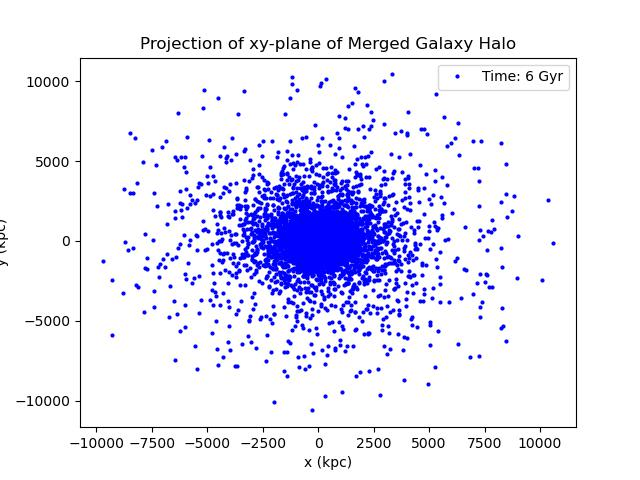
\includegraphics[width=\columnwidth]{xy-plane projection.jpg}
    \caption{Projection of the xy-plane of the merged DMH of the MW and M31, plotted such that the center of mass is at the origin. The data is from 6 Gyr after the beginning of the simulation and just after the merger has completed, corresponding to snapshot 420. This plot lacks an isodensity contour,and uses the low-resolution data for now.}                     
    \label{fig:xy-plane projection}
\end{figure}

There are few calculations that my code will need to be computed to retrieve the necessary data. A density profile must be fitted for the combined DMH remnant, so that the edge of the halo can be determined. Using the \textbf{Hernquist Profile} from \citet{Hernquist_1990}, we will determine a density profile, fitting an isodensity contour to determine the halo edge. The Hernquist Profile is defined as equation (\ref{hernquist}), where \begin{math}M_{halo}\end{math} is the total mass of the DMH, \begin{math}h_a\end{math} is the scale radius of the Hernquist profile, and \begin{math}r\end{math} is the distance from the galactic center. Minimal calculation is needed from here. The virial radius will be found using the Hernquist profile.

\begin{equation} \label{hernquist}
    \rho(r)=\frac{M_{halo}}{2\pi} \frac{h_a}{r(r+h_a)^3}
\end{equation}


The data will be plotted in many different forms to visualize the dark matter distribution. Projections of the xy, xz, and yz-planes of the DMH will be plotted with an ellipse fit to the isodensity contour that agrees with the virial radius, to visualize the ellipticity of the DMH. The axis ratios will be used to determine its shape. Finding the axis ratios for the DMH for each snapshot after the merger has completed will allow for an analysis of the evolution of the shape. By graphing how the axis ratio changes overtime, we can show how its shape evolves immediately after the merger.

From \citet{Despali_2016} a shape elongated along the merger axis is expected. Radiative processes, star formation, and AGN feedback are absent in this simulation. These processes generally smooth the halo to create a more oblate shape, so the simulation is expected to favor a non-oblate shape. Further, because these halos are so large, we expect the growth of the halo to begin with an initially triaxial shape. Combining the above, a triaxial halo with its longest axis in the direction of the merger axis is expected as the merged halo shape.


%%%%%%%%%%%%%%%%%%%% REFERENCES %%%%%%%%%%%%%%%%%%

% The best way to enter references is to use BibTeX:

\bibliographystyle{mnras}
\bibliography{example} % if your bibtex file is called example.bib


% Alternatively you could enter them by hand, like this:
% This method is tedious and prone to error if you have lots of references
%\begin{thebibliography}{99}
%\bibitem[\protect\citeauthoryear{Author}{2012}]{Author2012}
%Author A.~N., 2013, Journal of Improbable Astronomy, 1, 1
%\bibitem[\protect\citeauthoryear{Others}{2013}]{Others2013}
%Others S., 2012, Journal of Interesting Stuff, 17, 198
%\end{thebibliography}

%%%%%%%%%%%%%%%%%%%%%%%%%%%%%%%%%%%%%%%%%%%%%%%%%%

%%%%%%%%%%%%%%%%% APPENDICES %%%%%%%%%%%%%%%%%%%%%



% Don't change these lines
\bsp	% typesetting comment
\label{lastpage}
\end{document}

% End of mnras_template.tex
